\section{Background and Motivation}

In this section, we provide the background and motivation for this work.

\subsection{Graph Vertex Processing}

\begin{figure}[htbp]
\centering
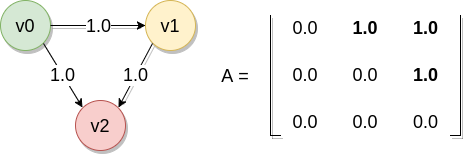
\includegraphics[width=0.5\textwidth]{figures/sample_graph}
\caption{Sample Graph Representation}
\label{fig:sample_graph}
\end{figure}

\begin{figure}[htbp] 
\begin{equation}
\#Edges = A^{T} \times Identity
\end{equation}
\begin{equation}
\#Edges = 
\left(\begin{array}{ccc} 0 & 0 & 0 \\ 1 & 0 & 0 \\ 1 & 1 & 0 \end{array}\right) \times
\left(\begin{array}{c} 1 \\ 1 \\ 1 \end{array}\right) 
= \left(\begin{array}{c} 0 \\ 1 \\ 2 \end{array}\right) 
\end{equation}
\caption{Incoming Edges Algorithm}
\label{fig:sample_algorithm}
\end{figure} 

\begin{lstlisting}[
	emph={Assign, Process, Apply}, emphstyle=\color{blue}, 
	numbers=none, 
	escapechar=\%, 
	caption=Graph Vertex Processing Model,
	label={lst:vertex_model}]
GraphProgram(%\textit{G}%, %\textit{P}%, %\textit{N}%) :
  for_each %\textit{N}% :
    x := Assign(%\textit{P}%)
  	y := Process(%\textit{G}%,x)
  	%\textit{P}% := Apply(%\textit{P}%,y)	  
  
e.g. FindIncomingEdges(%\textit{G}%=A, %\textit{P}%=%\textit{\textbf{I}}%, %\textit{N}%=1) :
           Assign(%\textit{P}%)    := %\textit{P}%
     where Process(%\textit{G}%,x) := %\textit{G}% * x
           Apply(%\textit{P}%,y)   := y
\end{lstlisting}

A large variety of programming models have been proposed for describing Graph algorithms, expressing computation using vertex operations on matrices \cite{GraphMat} \cite{GraphLab}, \cite{Pregel}, \cite{MapGraph} \cite{GraphX} task-based models \cite{Galois} or domain-specific languages \cite{GreenMarl}. The vertex programming model has show great adoption for its ease of abstraction for describing algorithms using Linear Algebra and its efficient computation on commodity multi-core processors.

Figure \ref{fig:sample_graph} shows a simple 3 vertices graph example with its corresponding 3x3 matrix representation. For every edge between a source and destination vertex, the corresponding row and column entry in the matrix is activate. For instance, the matrix entry in row 0 and column 1 represents the edge between source \textit{v0} and destination \textit{v1}. using the matrix representation, we can apply an algorithm on the graph to calculate the total number of incoming edges at each vertex. This algorithm can be expressed using a simple matrix-vector operation as shown in equations (1) and (2) in Figure \ref{fig:sample_algorithm}. Several graph algorithms, including Breadth First Search (BFS) \cite{BFS}, PageRank \cite{PageRank}, Single Source Shortest-Path (SSSP) \cite{SSSP}, can be described similarly using the vertex programming model \cite{GraphMat}.

Listing \ref{lst:vertex_model} shows the three stages of a generalized graph vertex processing model - \textit{Assign}, \textit{Process} and \textit{Apply}, given a graph \textit{G}, some vertex properties \textit{P} and an iteration count \textit{N}. The \textit{Assign} stage generates an input vector \textit{x} using the vertex properties \textit{P}. The \textit{Process} stage applies the input vector \textit{x} to the graph \textit{G} and generates an output vector \textit{y}. The\textit{ Apply} gather the resulting output vector to update the vertex properties for the next iteration. The graph program executes the three stages for several iterations until it converges. A direct mapping of our incoming edges algorithm to this processing model is also provided in Listing 1, where the identity vector is used for the vector properties. The \textit{Assign} and \textit{Apply} stages of this program are simple identity operators, while the \textit{Process} stage perform a matrix-vector multiplication. The input graph can be represented as a compressed sparse matrix to only store the non-zero entries of the graph. This data structure enables accelerated computation, often using a Sparse Matrix-Sparse Vector Multiplication (SpMSpV) kernel to target multi-core CPUs \cite{GraphMat} or GPUs \cite{MapGraph}. The computation that cannot be accelerated is simply executed on the general-purpose host CPU. FlexGraph's objective is to provide a more energy efficient graph processing backend using a FPGA for hardware acceleration \cite{Catapult}.

\subsection{Intel Heterogeneous CPU-FPGA Platform}

\begin{figure}[htbp]
\centering
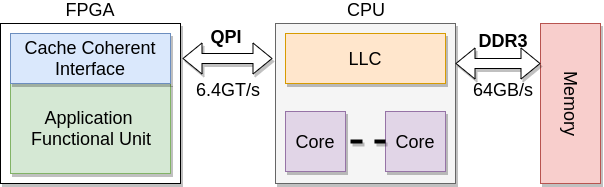
\includegraphics[width=0.5\textwidth]{figures/harp_arch}
\caption{Intel HARP Architecture}
\label{fig:harp_arch}
\end{figure}

With the rising adoption of FPGAs in production data centers \cite{Catapult}, there is a need to increase its ecosystem by making them more energy efficient as well as accessible to both the users and designers. Modern CPU-FPGA platforms \cite{CPU-FPGA} provide tightly-coupled shared-memory CPU-FPGA integration \cite{CAPI} \cite{CCI}, making then easier to program and efficient for hardware acceleration. Figure \ref{fig:harp_arch} shows an overview architecture of the Intel Xeon-FPGA platform prototype that we used in our evaluation. It has a dual-socket system, one containing a 10-core Intel Xeon E5-2680 CPU and the other containing an Altera Stratix V 5SGXEA FPGA operating at 200 MHz. The two sockets are connected via a 6.4 GT/s QPI \cite{QPI} link for data transfer. The FPGA's area is partitioned into two main blocks - the Application Function Unit (AFU) or 'Green' bitstream allocated for the custom accelerator and the 'Blue' bitstream implementing the Cache Coherent Interface (CCI) for the accelerator. The CCI runtime implements a 64 KB direct-mapped cache to support address translation (1024 page table entries) with request re-ordering for a total of 2 GB of addressable memory. The AFU memory interface is 64-byte cache-line addressable and it is up to the accelerator to extend the interface if fine grained (e.g. single byte) access is desired.

\subsection{Collaborative CPU-FPGA Computation}

\begin{figure}[htbp]
\centering
\begin{subfigure}{0.25\textwidth}
    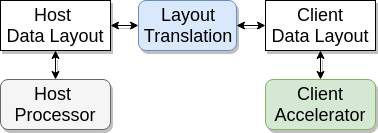
\includegraphics[width=\textwidth]{figures/offload_model}
    \caption{Offload model}
    \label{fig:offload_model}
\end{subfigure}
\hfill
\begin{subfigure}{0.21\textwidth}
    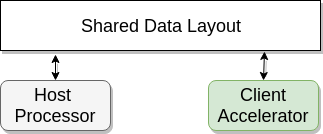
\includegraphics[width=\textwidth]{figures/collaborative_model}
    \caption{Collaborative model}
    \label{fig:collaborative_model}
\end{subfigure}
\caption{Shared Memory Compute Models}
\label{fig:compute_model}
\end{figure}

The prevalent execution model for accelerator design is the offload model \cite{Accelerators} where computation takes place on discrete copies of a shared resource that are optimized for efficient access by the target device. In this model of computation, the host processor applies some layout translation on the data before making it available to the client accelerator (see Figure \ref{fig:offload_model}). The additional latency of the translation process is generally mitigated using optimization techniques such as batching and double-buffering. The offload model is well suited for discrete memory systems where the necessary data transfer can be coupled with layout translation. One attractive application of shared-memory systems is the enabling of efficient collaborative computation (see Figure \ref{fig:collaborative_model}) in which all attached compute elements can access the same shared resource and modifying it during the course of the program execution. It is particularly ideal if the data layout provides efficient access by the compute devices. Contrarily to existing Graph Analytics Accelerators \cite{Graphicionado} \cite{GraphOps} that employ a custom optimized graph data structure for computation, Flexgraph uses a sparse matrix format for computation. This decision provides several advantages - first, it is storage efficient because the graph's physical memory is shared - second, it enables collaborative computation with the host CPU, leveraging the large ecosystem of matrix-based frameworks \cite{CombBlas} \cite{Pegasus} - third, it decouples the software and hardware design, enabling them to scale independently.

\section{FlexGraph Architecture}

In this section, we describes the overall architecture of the FlexGraph Accelerator.

\subsection{The DCSC Matrix Format}

\begin{figure}[htbp]
\begin{subfigure}{0.5\textwidth}
    \includegraphics[width=\textwidth]{figures/csc_format}
    \vspace{0pt}
\end{subfigure}
\begin{subfigure}{0.33\textwidth}
    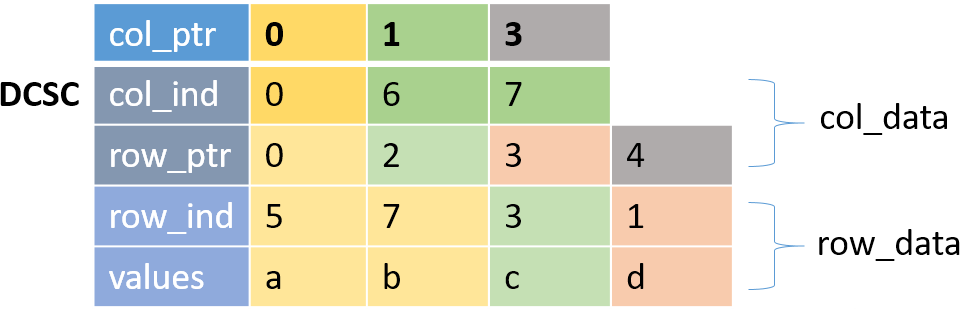
\includegraphics[width=\textwidth]{figures/dcsc_format}
\end{subfigure}
\caption{Matrix formats comparison}
\label{fig:DCSC_matrix_format}
\end{figure}

FlexGraph uses the Doubly Compressed Sparse Column (DCSC) \cite{DCSC} format as underlying graph data structure. The format allows minimal traversal into the sparse matrix structure, saving necessary memory bandwidth when fetching empty columns. Figure \ref{fig:DCSC_matrix_format} shows the memory layout for a sample matrix A = \{(0,5,a), (0,7,b), (6,3,c), (7,1,d)\} with four non-zero edges (src, dst, weight) encoded using DCSC versus the conventional CSC \cite{CSC} format. The traversal over CSC requires accessing all consecutive column ranges \textit{(cols[i+2] - cols[i])} even though most of the distances are empty. DCSC saves on bandwidth by using an additional indirection  buffer inside its structure to only encode non-zero columns. It is important to note that this indirection can introduce additional storage overhead and access latency if the matrix is too small or not sparse enough. However, Graph Analytics datasets are generally very large and hyper-sparse which eliminate the DCSC format overhead. In addition to a sparse matrix, FlexGraph also uses a sparse vector to provide property data as well as edge selection during computation. A bitmask is used to encode the non-zero entries in the input vector.

\subsection{The Sparse Matrix-Sparse Vector Multiplication Kernel}

\begin{lstlisting}[
	linebackgroundcolor={
	\ifnum\value{lstnumber}=6\color{red!10}\fi
	\ifnum\value{lstnumber}=8\color{red!10}\fi
	\ifnum\value{lstnumber}=5\color{orange!10}\fi
	\ifnum\value{lstnumber}=10\color{orange!10}\fi}, 
    escapechar=\%, 
    emph={col_ind, col_ptr, row_ind, row_ptr, a_val}, emphstyle=\color{blue}, 
    caption=Pseudo-code for SpMSpV kernel,
    label={lst:spmv_code}]
def SpMSpV_kernel(a, x):
  y_values[] = {0}
  y_bitmask[] = {false}
  for_each i in a.col_ptr
    (col_ind, row_ptr) := a.col_data[i]
    x_active = x.bitmask[col_ind]          
    if (x_active):                            
      x_val = x.values[col_ind]              
      for_each j in row_ptr
        (row_ind, a_val) := a.row_data[j]
        y_values[row_ind] += a_val * x_val
        y_bitmask[row_ind] = true          
  return (y_values, y_bitmask)
\end{lstlisting}

FlexGraph micro-architecture implements a Sparse Matrix-Sparse Vertex Multiplication (SpMSpV) kernel in FPGA. This kernel diverges from conventional Sparse Matrix-Vector Multiplication (SpMV) implementations in two ways - firstly, it uses a sparse data structure as input and output vector during computation - secondly, it uses a doubly-compressed sparse matrix (DCSC) format with additional memory indirection buffer when accessing the matrix columns. These two properties present unique performance challenges when designing the accelerator. Listing \ref{lst:spmv_code} shows the pseudo-code of the SpMSpV kernel. Given the start/end addresses (col\_start, col\_end) into the matrix columns buffer (coldata), for The program iterates through each column entry and fetches the corresponding column index (col) and rows buffer address (row\_start, row\_end). It then checks if the current column index (col) is active using the vertex bitmask, only then it proceeds with rows traversal loop where the matrix row\_data is accessed to retrieve corresponding row index and matrix value for computation. A Multiply-Accumulate (MAC) operation is then performed on the matrix and vertex data and output bitmask is updated. Lines 6 and 8 show the code region where external memory is randomly accessed to obtain the vertex data and active state. Lines 5 and 10 show the code region where external memory is accessed semi-random because only the first access cannot be predicted and after that the address is simply incremented. FlexGraph's architecture attempts to address some of those performance hogs using several optimizations detailed in section 4.

\subsection{FlexGraph Microarchitecture}

\begin{figure}[htbp]
\centering
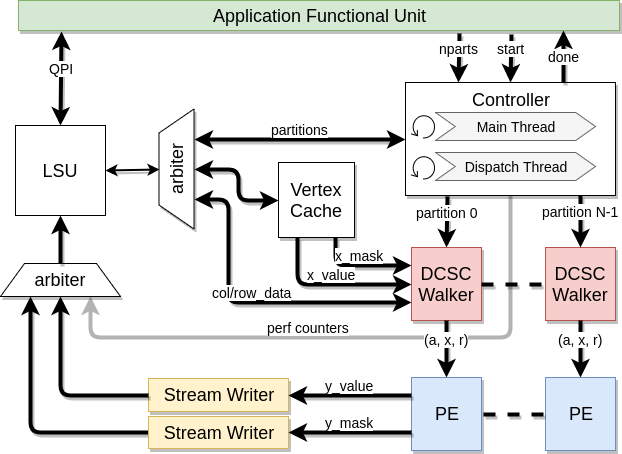
\includegraphics[width=0.5\textwidth]{figures/microarchitecture}
\caption{FlexGraph Microarchitecture}
\label{fig:microarchitecture}
\end{figure}

Figure \ref{fig:microarchitecture} illustrates the microarchitecture of FlexGraph accelerator. Externally, FlexGraph input and output ports implement an Accelerator Functional Unit (AFU) interface defined by Intel's Accelerator Abstraction Layer (AAL) \cite{Intel-FPGA}. AFUs implementing the interface are able to bind with the FPGA's board support package (BSP) and seamlessly communicate with the AAL runtime on the host processor. The interface exposes four signals \textit{qpi, ctx, start, done}, where the \textit{qpi} bus handles shared-memory communications, \textit{ctx} is used for passing custom input context to the accelerator, in our case we pass down all data structure layout information needed to access memory, \textit{start} and \textit{done} are the control knobs for starting and ending execution. At a high-level, Flexgraph's
microarchitecture consists for a six building blocks: The main controller, the DCSC matrix walkers, the processing elements, the stream writers, the vertex caches and the load/store unit (LSU). 

\subsection{Main Controller}

Upon reception of the \textit{start} signal from the host processor, the main controller is responsible for scheduling matrix partitions for execution on each processing element. It is comprised of two execution threads: A request thread that fetches partition data from the load/store unit into a local buffer, a dispatch thread that submit received partition data to individual matrix walker engines for processing. After all matrix partitions have been processed, the controller sends performance counters back to the host processor and activates the \textit{done} signal.

\subsection{DCSC Matrix Walkers}

\begin{figure}[htbp]
\centering
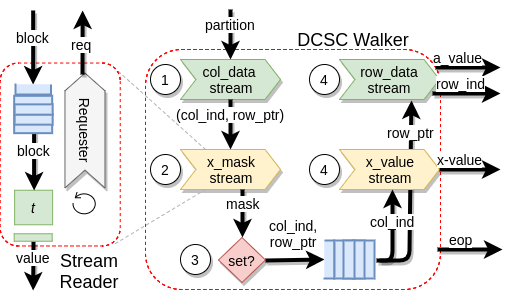
\includegraphics[width=0.5\textwidth]{figures/micro_walker}
\caption{DCSC Walker}
\label{fig:micro_walker}
\end{figure}

The DCSC Matrix Walker is a custom data structure traversal engine for the DCSC Matrix. Figure \ref{fig:micro_walker} shows an overview of the engine microarchitecture. It is implemented as a four-stage state machine where each stage accesses a portion of the matrix layout as reflected in the pseudo-code in Listing \ref{lst:spmv_code}. In the first stage, the engine fetches column data (\textit{col\_ind, row\_ptr}) from memory given the partition address. In the second stage, the engine fetches the vertex active mask from memory given the \textit{col\_ind} value obtained in the previous stage. In the third stage, the engine checks if the current property is active using the mask obtained in the previous stage, if so passes the associated column data to the next stage. In the fourth stage, the engine fetches the vertex data and the matrix row data (\textit{row\_ind, a\_val}) from memory for each active column data and send those values to the connected processing element where the actual computation takes place. Each fetch unit is implemented as a Stream Reader engine to handle coarse-grain memory access for the associated data. It consists of a request module for sending memory read access command, a fifo buffer for receiving requested blocks and a temporary block buffer for accessing sub-block elements. The vertex data (values, masks) are fetched from dedicated vertex caches to enable reuse by the walker engines. We use a crossbar to multiplex outgoing requests from the walker engines to the LSU and vertex caches.

\subsection{Processing Elements}

\begin{figure}[htbp]
\centering
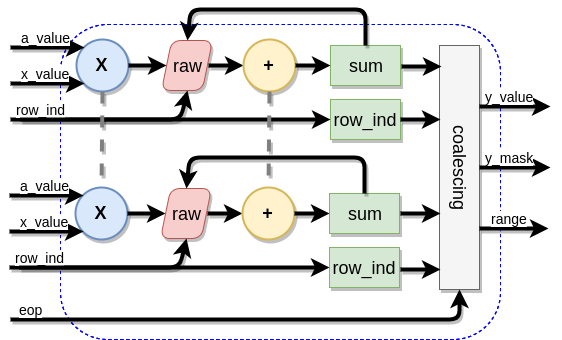
\includegraphics[width=0.5\textwidth]{figures/micro_pe}
\caption{Processing Element}
\label{fig:micro_pe}
\end{figure}

Figure \ref{fig:micro_pe} shows an overview of a processing element microarchitecture. It main objective is to perform a floating-point multiplication on the incoming vertex and matrix values from the connected walker engine and accumulate the result until the whole partition has been processed. It is comprised of eight parallel pipelined Multiply-Accumulate (MAC) units attached to a coalescing output module. Eight is the maximum number of matrix row data that can be stored in a single cache block. Each MAC lane consists of pipelined floating-point multiply module, a pipelined floating-point Add unit, a Read-After-Write (RAW) control unit that stalls the pipeline if the current \textit{row\_ind} is pending addition. We build a bitmask given the \textit{row\_ind} to track outstanding operations in addition units. The accumulated result is stored into a local buffer indexed by the \textit{row\_ind} value. Each processing element also computes the aggregate active rows mask for the given partition. At the end of the partition processing, the coalescing unit merges output values and masks according to their associated block address and sends the result to the Stream Writers.

\subsection{Stream Writers}

\begin{figure}[htbp]
\centering
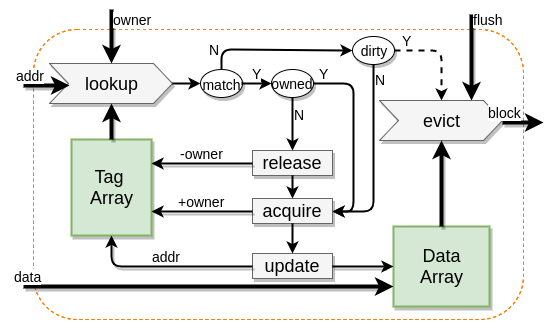
\includegraphics[width=0.5\textwidth]{figures/micro_writer}
\caption{Stream Writer}
\label{fig:micro_writer}
\end{figure} 

The Stream Writers are coalescing write buffers that batches write requests to memory until entire blocks are updated before they are submitted. We used two stream writers, one for the storing vertex output and one for storing the output mask. Figure \ref{fig:micro_writer} shows an overview of a stream writer microarchitecture. Internally, a stream writer has an architecture similar to a cache but has been augmented with block ownership information and the stored value is merged, not overwritten. It consists of four main modules: A data store, A tag store, and lookup unit and an eviction unit. The data store holds all the blocks sent to the device. The tag store keeps the meta-data associated with each block in the data store. A tag consists of the block address and an owners list. The owners list is implemented as a bitmask that tracks the processing elements currently using a given block. In a typical operation where the writer receives a block write request, the lookup unit is first invoked to find an existing entry for the corresponding block in the tag store. If there is a match and the block is already owned, the incoming value is simply merged with existing one. If a match was found, but the block is not owned, the previosuly owned block is released and this new one is acquired before data update. If no match is found, the device allocates a new block for the request and evicts existing data to memory if dirty. The writer also support an explicit flush command to the eviction of all dirty blocks to memory when all processing is completed.

\subsection{Vertex Caches}

FlexGraph uses two direct-mapped vertex caches to keep the vertex values and mask in the accelerator for reuse by the matrix walker engines. Their source port is connected to the load/store unit via an arbiter that multiplexes outgoing read requests with the controller and the matrix walkers. It has a typical cache architecture with an input buffer for tracking outstanding requests.

\section{FlexGraph Software-Hardware Codesign}

\begin{lstlisting}[language=C++, caption=AAL Device Interface in Cocoh C++]
class aal_device {
public: 
  virtual out_t initialize()(
    const ch_logic& start, 
    const qpi::in_t& qpi_in, 
    const afu_ctx_t& ctx, 
    qpi::out_t& qpi_out, 
    ch_logic& done
  ) const = 0;  
};
\end{lstlisting}